\documentclass[article,36pt,extrafontsizes,oneside,openany,oldfontcommands]{memoir}
% \usepackage{natbib}
% \bibliographystyle{/Users/kengchichang/Dropbox/BibDesk/bst/econ_aer}
\usepackage[backend=biber,
    loccittracker=true,
    abbreviate=false,
    citetracker=false,
    authordate,
    sorting=ynt,
    isbn=false,
    hyperref=true,
    url=true,
    doi=true,
    eprint=false,
    hyperref=true,
    sortcites=true]{biblatex-chicago}
\addbibresource{/Users/kengchichang/Dropbox/Zotero/bib/all_papers_zotero.bib}
\AtBeginBibliography{\small}
\setlength{\bibitemsep}{0.0pt}
\setlength{\bibhang}{0.0pt}

\usepackage[export]{adjustbox}
\usepackage{wrapfig}

\usepackage{graphicx}
    \graphicspath{{figure/}}
\usepackage{amsmath, amsfonts, amssymb, amsthm}
\usepackage{mathtools}
\usepackage[charter,expert]{mathdesign}
\usepackage{fontspec}
\usepackage{xltxtra, xunicode}
\usepackage[utf8]{inputenc}
\RequirePackage[CJKmath = true, 
                indentfirst = false, 
                PunctStyle = {quanjiao}, 
                CheckSingle = true, 
                SlantFont, 
                BoldFont]
                {xeCJK}
%\usepackage{lmodern}
%\usepackage{times}
%\usepackage{mathptmx}
%\usepackage[minionint, lf, mathtabular]{MinionPro}
\usepackage{bm}
\RequirePackage{lipsum}
\RequirePackage{blindtext}
\RequirePackage[svgnames,table]{xcolor}
\RequirePackage{tikz}
\RequirePackage[framemethod=tikz]{mdframed}
\RequirePackage{color}
\RequirePackage{geometry}
\RequirePackage{adjmulticol}
\RequirePackage[skins,most,listings,skins]{tcolorbox}

%For kable extra package :)
\RequirePackage{longtable}
\RequirePackage{array}
\RequirePackage{multirow}
\RequirePackage{wrapfig}
\RequirePackage{float}
\RequirePackage{colortbl}
\RequirePackage{pdflscape}
\RequirePackage{pagecolor}
\RequirePackage{tabu}
\RequirePackage{threeparttablex}
\RequirePackage[normalem]{ulem}
\RequirePackage{makecell}
\RequirePackage{wrapfig}
\usepackage{xmpmulti, booktabs, multicol}
\usepackage{threeparttable}
\usepackage{dcolumn}
\newcolumntype{.}[1]{D{.}{.}{#1}}
\newcolumntype{,}[1]{D{,}{,}{#1}}
\usepackage{siunitx}
\sisetup{%
  mode = math,
  detect-all,  
  output-decimal-marker = {.},
  group-separator = {,},
  math-rm = \rmnumeric,
  text-rm = \rmnumeric,
}

%rof hyperrefs
\usepackage{color}
    \definecolor{MyBrown}{HTML}{3D3D00}
    \definecolor{MyBlue}{HTML}{003A75}  
    \definecolor{MyRed}{HTML}{6F1A2F}
    \definecolor{MyGreen}{HTML}{004847}
\usepackage{hyperref}
    \hypersetup{bookmarks = true,
                bookmarksnumbered = true,
                colorlinks = true,
                linkcolor = MyRed,
                citecolor = MyBlue, % hyperref is in conflict with natbib
                filecolor = MyBrown,
                urlcolor = MyGreen}
%For figure and table placement
\RequirePackage{float}
\floatplacement{figure}{H}
\floatplacement{table}{H}

%%%%%%%%% COLOURS %%%%%%%%
%Fill/ Line Colours
\definecolor{titleboxbgcol}{HTML}{D8E0FF}
\definecolor{titleboxbordercol}{HTML}{205DA4}
\definecolor{columnlinecol}{HTML}{008080}
\definecolor{bodybgcol}{HTML}{ffffff}
\definecolor{sectitlebgcol}{HTML}{D8E0FF}
\definecolor{sectitlebordercol}{HTML}{D8E0FF}
% Text Colours
\definecolor{titletextcol}{HTML}{1c518f}
\definecolor{authortextcol}{HTML}{000000}
\definecolor{affiliationtextcol}{HTML}{000000}
\definecolor{sectitletextcol}{HTML}{1c518f}
\definecolor{bodytextcol}{HTML}{000000}
\definecolor{footnotetextcol}{HTML}{000000}
\definecolor{citecol}{HTML}{CC0000}
\definecolor{urlcol}{HTML}{008080}
\definecolor{linkcol}{HTML}{008080}


%Memoir spacing options
%spacing between figure/ table and caption
\setlength{\abovecaptionskip}{0.4in}
\setlength{\belowcaptionskip}{0.2in}
\captionnamefont{\large}
\captiontitlefont{\large}

%define column options
\setlength{\columnseprule}{0pt}
\def\columnseprulecolor{\color{columnlinecol}}

%define section title features
\setsubsubsecheadstyle{\small\color{sectitletextcol}\textbf}% Set \section style
\setsecnumformat{}
\def\sectionmark#1{\markboth{#1}{#1}}

%%%%%%%%%%%% TCOLORBOXES TO THE RESCUE %%%%%%%%%%%%%%%%%%%%
%Title Box
\newtcolorbox{topbox}{
enhanced,
colback=titleboxbgcol,
colframe=titleboxbordercol,
halign=center,
boxrule=0cm,
sharp corners=all,
 overlay={
    % \node[anchor=south west]
    %   at ([xshift=1in,yshift=1in]frame.south west)
    %    {\includegraphics[width=3in]{Figures/posterdownlogo}};
    % \node[anchor=south east]
    %   at ([xshift=-1in,yshift=1in]frame.south east)
    %    {\includegraphics[width=3in]{Figures/posterdownlogo}};
       }

}
%Body Section Title Box
\newtcolorbox{myboxstuff}[1][]{
code={\parindent=0em},
colframe=sectitlebordercol,
nobeforeafter,
left skip=0pt,
valign=center,
halign=center,
fontupper=\large\bfseries,
colupper=sectitletextcol,
boxrule=2mm,
colback=sectitlebgcol,
sharp corners=south, #1}
\newcommand{\mybox}[1]{%
\begin{myboxstuff}
\strut #1
\end{myboxstuff}%
}
\makeheadstyles{MyBox}{
    \setsecheadstyle{\mybox}
}
\headstyles{MyBox}\makepagestyle{MyBox}
%-----------------------------------------------------
%Make sure that the page is empty of any preset items from memoir
\thispagestyle{empty}

%biblatex options
%\usepackage{natbib}
%\DeclareTextCommandDefault{\nobreakspace}{\leavevmode\nobreak\ } % AER style nobreak
\renewcommand{\bibname}{\hrule}
%\renewcommand{\bibsection}{}
%\renewcommand*{\bibfont}{\fontsize{40pt}{45pt}\selectfont}
%\setlength{\bibsep}{0pt plus 0.3ex}

%Remove section numbering & set 2nd level header as first level
%to avoid the automatic new page generated from memoir chapter
%formatting
\counterwithout{section}{chapter}
\makechapterstyle{mydefault}{
\addtocounter{secnumdepth}{2}
\setsecheadstyle{\mybox}
\setsubsecheadstyle{\itshape}
\setsubsubsecheadstyle{\itshape}
}

%set the chapterstyle
\chapterstyle{mydefault}

%define column spacing
\setlength\columnsep{0.5in}

%spacing params
\setlength\parindent{0em}
\setlength\parskip{0em}
\setlength\hangparas{0em}

%spacing after section head title
\setaftersecskip{0em}
\setbeforesecskip{0.5em}
\setlength\textfloatsep{0in} % distance between floats on the top or the bottom and the text
\setlength\floatsep{0.1in} % distance between two floats
\setlength\intextsep{0.5in} % distance between floats inserted inside the page text (using h) and the text proper
\makeatletter
\g@addto@macro{\normalsize}{%
%    \setlength\abovedisplayskip{30pt} % spacing above equations
%    \setlength\abovedisplayshortskip{15pt} % spacing immediately above equations
%    \setlength\belowdisplayskip{0pt} % spacing below equations
%    \setlength\belowdisplayshortskip{0pt} % spacing immediately below equations
%    \setlength{\displayindent}{0in}
%    \setlength{\predisplaysize}{0in}
    } 
\makeatother

\setstocksize{36in}{48in}
\settrimmedsize{\stockheight}{\stockwidth}{*}
\settypeblocksize{36in}{48in}{*}
\setlrmargins{*}{*}{1}
\setulmarginsandblock{2.5cm}{0cm}{*}
\setmarginnotes{0em}{0cm}{0cm}
\setlength{\footskip}{0cm}
\setlength{\footnotesep}{0cm}
\setlength{\headheight}{0pt}
\setlength{\headsep}{0pt}
\setlength{\trimtop}{0pt}
\setlength{\trimedge}{0pt}
\setlength{\uppermargin}{0pt}
\checkandfixthelayout
\usepackage{enumitem}
\usepackage{bbm}
\usepackage{dsfont}
\def\one{\mathrm{1}\hspace{-12pt}\mathrm{1}}
\setlist[enumerate]{topsep=0pt,itemsep=-1ex,partopsep=1ex,parsep=1ex,leftmargin=2ex}
\setlist[itemize]{topsep=0pt,itemsep=-1ex,partopsep=1ex,parsep=1ex,leftmargin=2ex}

%Footnote to white
\RequirePackage{footmisc}
\def\footnotelayout{\centering\color{footnotetextcol}}

% see https://stackoverflow.com/a/47122900
\usepackage{color}
\usepackage{fancyvrb}
\newcommand{\VerbBar}{|}
\newcommand{\VERB}{\Verb[commandchars=\\\{\}]}
\DefineVerbatimEnvironment{Highlighting}{Verbatim}{commandchars=\\\{\}}
% Add ',fontsize=\small' for more characters per line
\usepackage{framed}
\definecolor{shadecolor}{RGB}{248,248,248}
\newenvironment{Shaded}{\begin{snugshade}}{\end{snugshade}}
\newcommand{\AlertTok}[1]{\textcolor[rgb]{0.94,0.16,0.16}{#1}}
\newcommand{\AnnotationTok}[1]{\textcolor[rgb]{0.56,0.35,0.01}{\textbf{\textit{#1}}}}
\newcommand{\AttributeTok}[1]{\textcolor[rgb]{0.77,0.63,0.00}{#1}}
\newcommand{\BaseNTok}[1]{\textcolor[rgb]{0.00,0.00,0.81}{#1}}
\newcommand{\BuiltInTok}[1]{#1}
\newcommand{\CharTok}[1]{\textcolor[rgb]{0.31,0.60,0.02}{#1}}
\newcommand{\CommentTok}[1]{\textcolor[rgb]{0.56,0.35,0.01}{\textit{#1}}}
\newcommand{\CommentVarTok}[1]{\textcolor[rgb]{0.56,0.35,0.01}{\textbf{\textit{#1}}}}
\newcommand{\ConstantTok}[1]{\textcolor[rgb]{0.00,0.00,0.00}{#1}}
\newcommand{\ControlFlowTok}[1]{\textcolor[rgb]{0.13,0.29,0.53}{\textbf{#1}}}
\newcommand{\DataTypeTok}[1]{\textcolor[rgb]{0.13,0.29,0.53}{#1}}
\newcommand{\DecValTok}[1]{\textcolor[rgb]{0.00,0.00,0.81}{#1}}
\newcommand{\DocumentationTok}[1]{\textcolor[rgb]{0.56,0.35,0.01}{\textbf{\textit{#1}}}}
\newcommand{\ErrorTok}[1]{\textcolor[rgb]{0.64,0.00,0.00}{\textbf{#1}}}
\newcommand{\ExtensionTok}[1]{#1}
\newcommand{\FloatTok}[1]{\textcolor[rgb]{0.00,0.00,0.81}{#1}}
\newcommand{\FunctionTok}[1]{\textcolor[rgb]{0.00,0.00,0.00}{#1}}
\newcommand{\ImportTok}[1]{#1}
\newcommand{\InformationTok}[1]{\textcolor[rgb]{0.56,0.35,0.01}{\textbf{\textit{#1}}}}
\newcommand{\KeywordTok}[1]{\textcolor[rgb]{0.13,0.29,0.53}{\textbf{#1}}}
\newcommand{\NormalTok}[1]{#1}
\newcommand{\OperatorTok}[1]{\textcolor[rgb]{0.81,0.36,0.00}{\textbf{#1}}}
\newcommand{\OtherTok}[1]{\textcolor[rgb]{0.56,0.35,0.01}{#1}}
\newcommand{\PreprocessorTok}[1]{\textcolor[rgb]{0.56,0.35,0.01}{\textit{#1}}}
\newcommand{\RegionMarkerTok}[1]{#1}
\newcommand{\SpecialCharTok}[1]{\textcolor[rgb]{0.00,0.00,0.00}{#1}}
\newcommand{\SpecialStringTok}[1]{\textcolor[rgb]{0.31,0.60,0.02}{#1}}
\newcommand{\StringTok}[1]{\textcolor[rgb]{0.31,0.60,0.02}{#1}}
\newcommand{\VariableTok}[1]{\textcolor[rgb]{0.00,0.00,0.00}{#1}}
\newcommand{\VerbatimStringTok}[1]{\textcolor[rgb]{0.31,0.60,0.02}{#1}}
\newcommand{\WarningTok}[1]{\textcolor[rgb]{0.56,0.35,0.01}{\textbf{\textit{#1}}}}

% choose font family
\RequirePackage{etoolbox}
%\RequirePackage{unicode-math}
\defaultfontfeatures{Ligatures=TeX,Scale=MatchLowercase,Mapping=tex-text]}
\setsansfont{Myriad Pro}
\setmainfont{Myriad Pro}
%\setmathfont{Fira Math}
\setmonofont[Scale=0.85]{Iosevka Comfy}
\newfontfamily\compthick{Myriad Pro Semibold Condensed}
\newfontfamily\compthin{Myriad Pro Light Condensed}
\newfontfamily\comp{Myriad Pro Condensed}
\newfontfamily\thin{Myriad Pro Light}
\setCJKmainfont[BoldFont={Hiragino Mincho ProN W6}]{Hiragino Mincho ProN W3}
\setCJKsansfont[BoldFont={Hiragino Sans W6}]{Source Han Sans J}
\setCJKmonofont[BoldFont={Yuanti TC Regular}]{Hiragino Maru Gothic ProN W4}

% define the BODYBGCOL
\newpagecolor{bodybgcol}

%sets footnote to be white hopefully
\renewcommand\footnoterule{}
\renewcommand{\thempfootnote}{\footnotesize\color{footnotetextcol}{\arabic{mpfootnote}}}

%include arbitrary input from header-includes field

%-------------- Begin Document -------------------%
\begin{document}

%-------------- Title Box Start ------------------%
%tcolorbox allows for pictures hopefully
\begin{topbox}
  \color{titletextcol}
  \vspace{0.8in}
  \bfseries
  \fontsize{100pt}{100pt}\selectfont
  {Mapping~~Visual~~Themes~~among~~Authentic~~and~~Coordinated~~Memes}\\[0.5in]  %% SC
  \color{authortextcol} 
  \mdseries
  \Large{Keng-Chi Chang~~$\cdot$~~UC San Diego~~$\cdot$~~\texttt{kechang@ucsd.edu}~~$\cdot$~~\texttt{kengchichang.com}~~$\cdot$~~2022 PolMeth at WUSTL} 
  % \\[0.2in] %% SC
  % \color{affiliationtextcol} \large{UC San Diego} %% SC
  \vspace{0.6in}
\end{topbox}


%--------------- Title Box End -------------------%
%----------------- Body Start --------------------%
% Begin body of poster


\fontsize{40pt}{45pt}\selectfont

\begin{adjmulticols*}{3}{0.5in}{0.5in}
\color{bodytextcol}

\section{Background \& Research Question}

\begin{adjustwidth}{0in}{0in}
\begin{itemize}[topsep=0pt,itemsep=0ex,partopsep=0ex,parsep=0ex]
\item Russian IRA shared 1.8M images on Twitter during 2016 election
\item Validated US Twitter users, 19\% tweets are memes, 30\% political
\item What distinguishes state-linked memes from authentic ones?
\end{itemize}
\end{adjustwidth}


\section{Data Collections}

\begin{adjustwidth}{0in}{0in}
\begin{itemize}[topsep=0pt,itemsep=0ex,partopsep=0ex,parsep=0ex]
\item 26K authentic memes from \texttt{r/meme} subreddit (authentic memes)
\item 15K non-meme image-with-text data (COCO-Text) as negative sample for training (so not simply a classifier for images with or without text)
\item 26K images from IRA on Twitter (coordinated memes if classified as meme)
\end{itemize} 
\end{adjustwidth}


\section{Methods Overview}
\begin{adjustwidth}{0.1in}{0in}
\begin{enumerate}[topsep=0pt,itemsep=0ex,partopsep=0ex,parsep=0ex]
\item Classify IRA images into memes vs. non-memes (test accuracy $>0.97$)
\item Extract visual embeddings jointly for both authentic memes (Reddit) and coordinated memes (IRA) using DeepCluster \href{http://arxiv.org/abs/1807.05520}{(Caron et al. 2019)}\\
{\centering 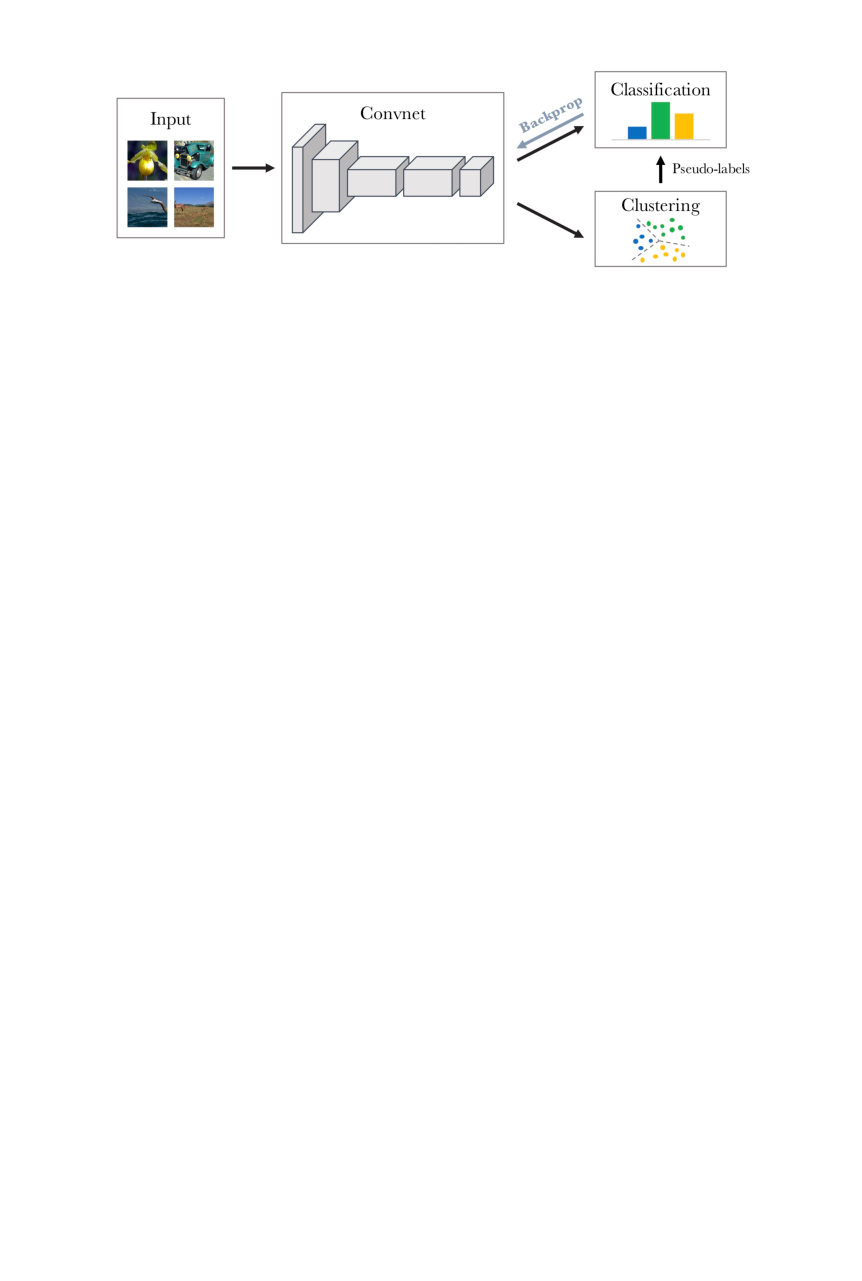
\includegraphics[width=.8\linewidth]{figure/deep_cluster.pdf}}
\item Cluster memes based on visual embeddings using K-means 
\item Label the clusters and compare between authentic/coordinated
\end{enumerate} 
\end{adjustwidth}



\section{Summary of Findings}
\begin{adjustwidth}{0.1in}{0in}
\begin{itemize}[topsep=0pt,itemsep=0ex,partopsep=0ex,parsep=0ex]
\item Latent visual embeddings reveal similarity between memes
\item Authentic and coordinated memes share most visual themes
\item Coordinated IRA memes more military, gender, quotes
\item Authentic Reddit memes more movie characters, comics
\item IRA accounts are not widely utilizing popular meme schemes in the US
\item Logistic regression on visual embedding discern IRA with $F_1=0.84$
\end{itemize} 
\end{adjustwidth}


\section{Example Clusters}
\begin{adjustwidth}{0.1in}{0in}
\begin{figure}
    \includegraphics[width=\linewidth]{figure/cluster_31_half.pdf}
    \\[1cm]
    \includegraphics[width=\linewidth]{figure/cluster_93_half.pdf}
\end{figure}
\vspace{-3cm}
\end{adjustwidth}

\columnbreak

% \begin{minipage}{.32\textwidth}
  \begin{figure}
    \vspace{2cm} \hspace{2.5cm} 
    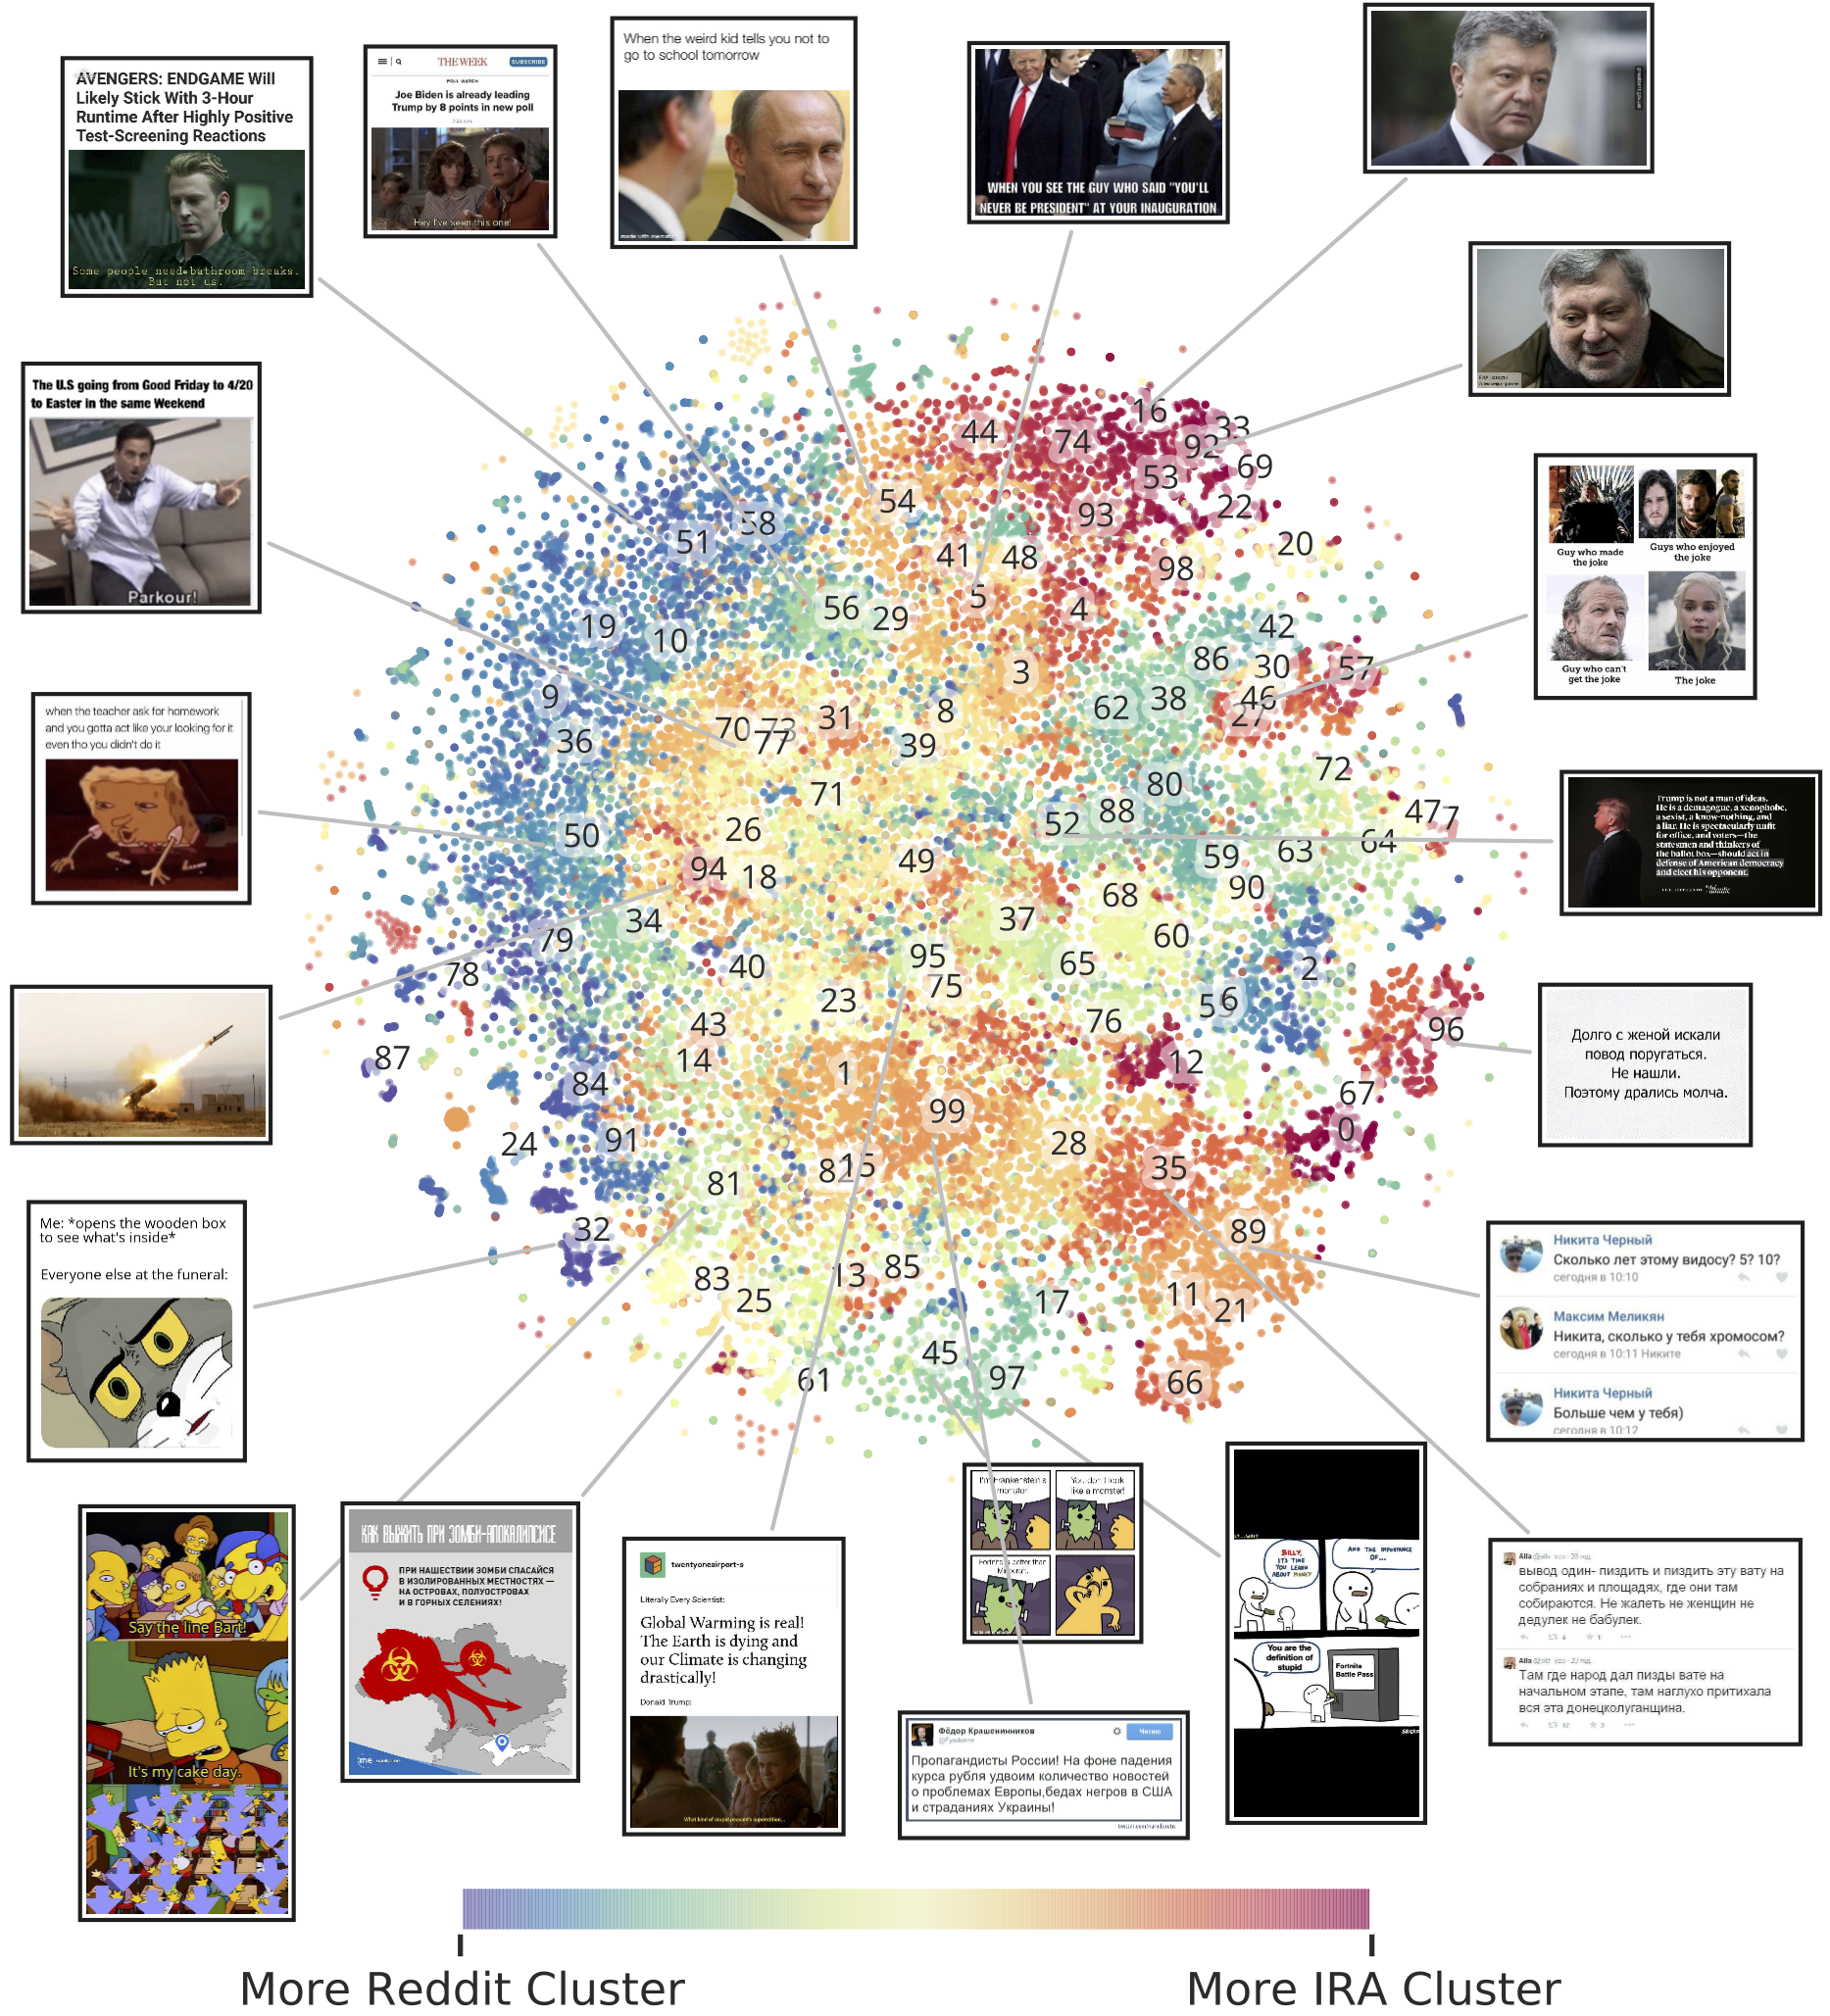
\includegraphics[width=1.25\linewidth]{figure/meme-cluster-tsne-rank-annotated.png}
  \end{figure}
% \end{minipage}


\begin{adjustwidth}{0.1in}{0in}
\vspace{1.25cm}
\begin{figure}
    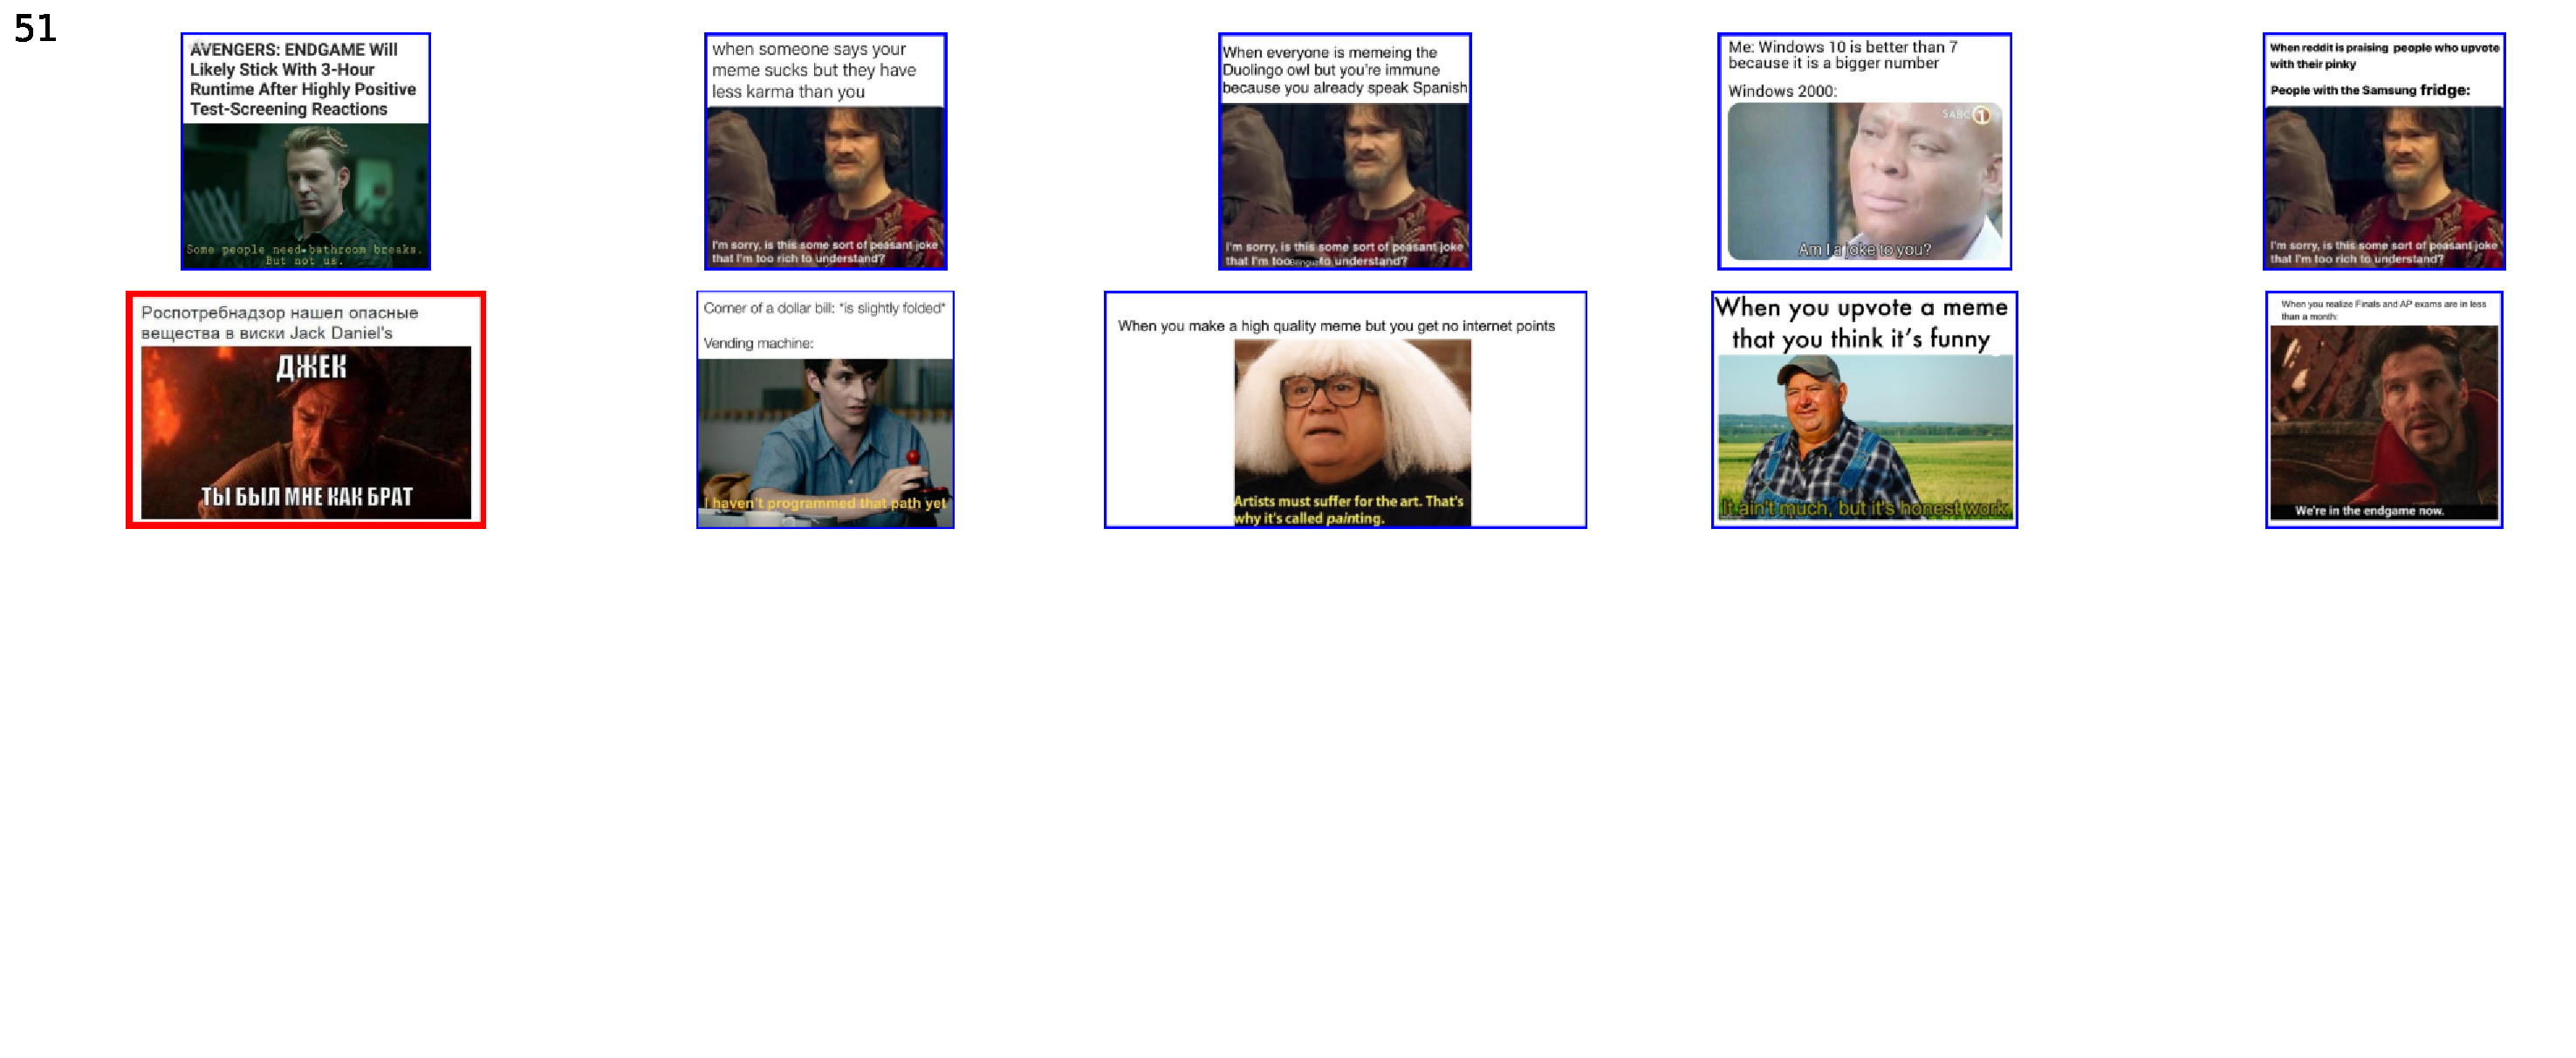
\includegraphics[width=\linewidth]{figure/cluster_51_half.pdf}
    \\[1cm]
    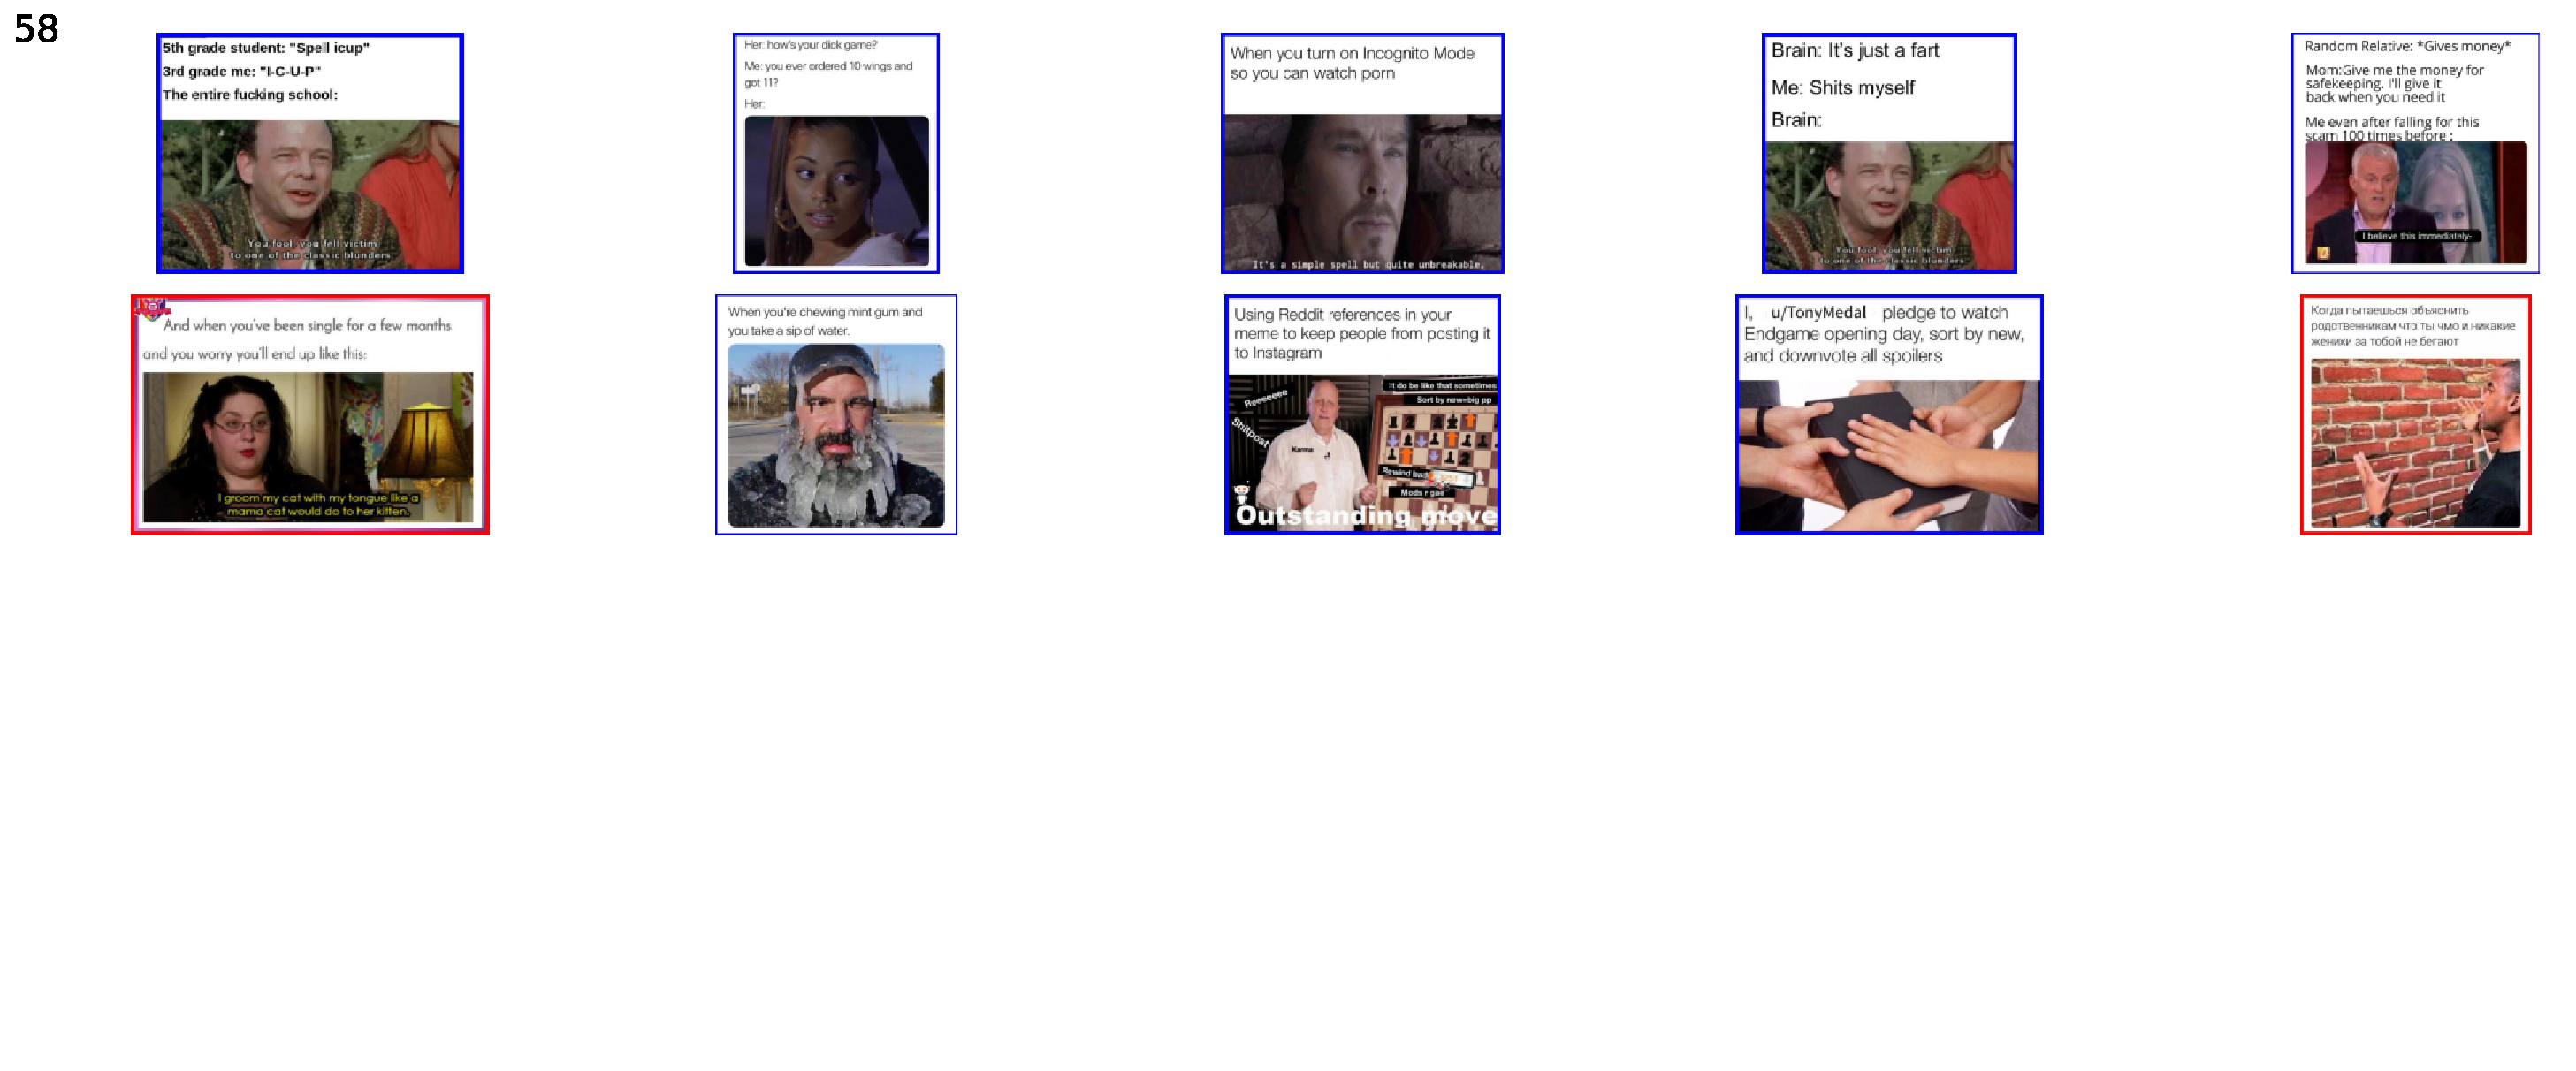
\includegraphics[width=\linewidth]{figure/cluster_58_half.pdf}
\end{figure}
\vspace{-3cm}
\end{adjustwidth}


\columnbreak


% \begin{minipage}{.2\textwidth}
  \begin{figure}
    %\centering
    \hspace{2cm}
    
\includegraphics[width=.15\linewidth]{figure/qr_code.png}
    %Comments/feedbacks
    \hspace{5cm}
    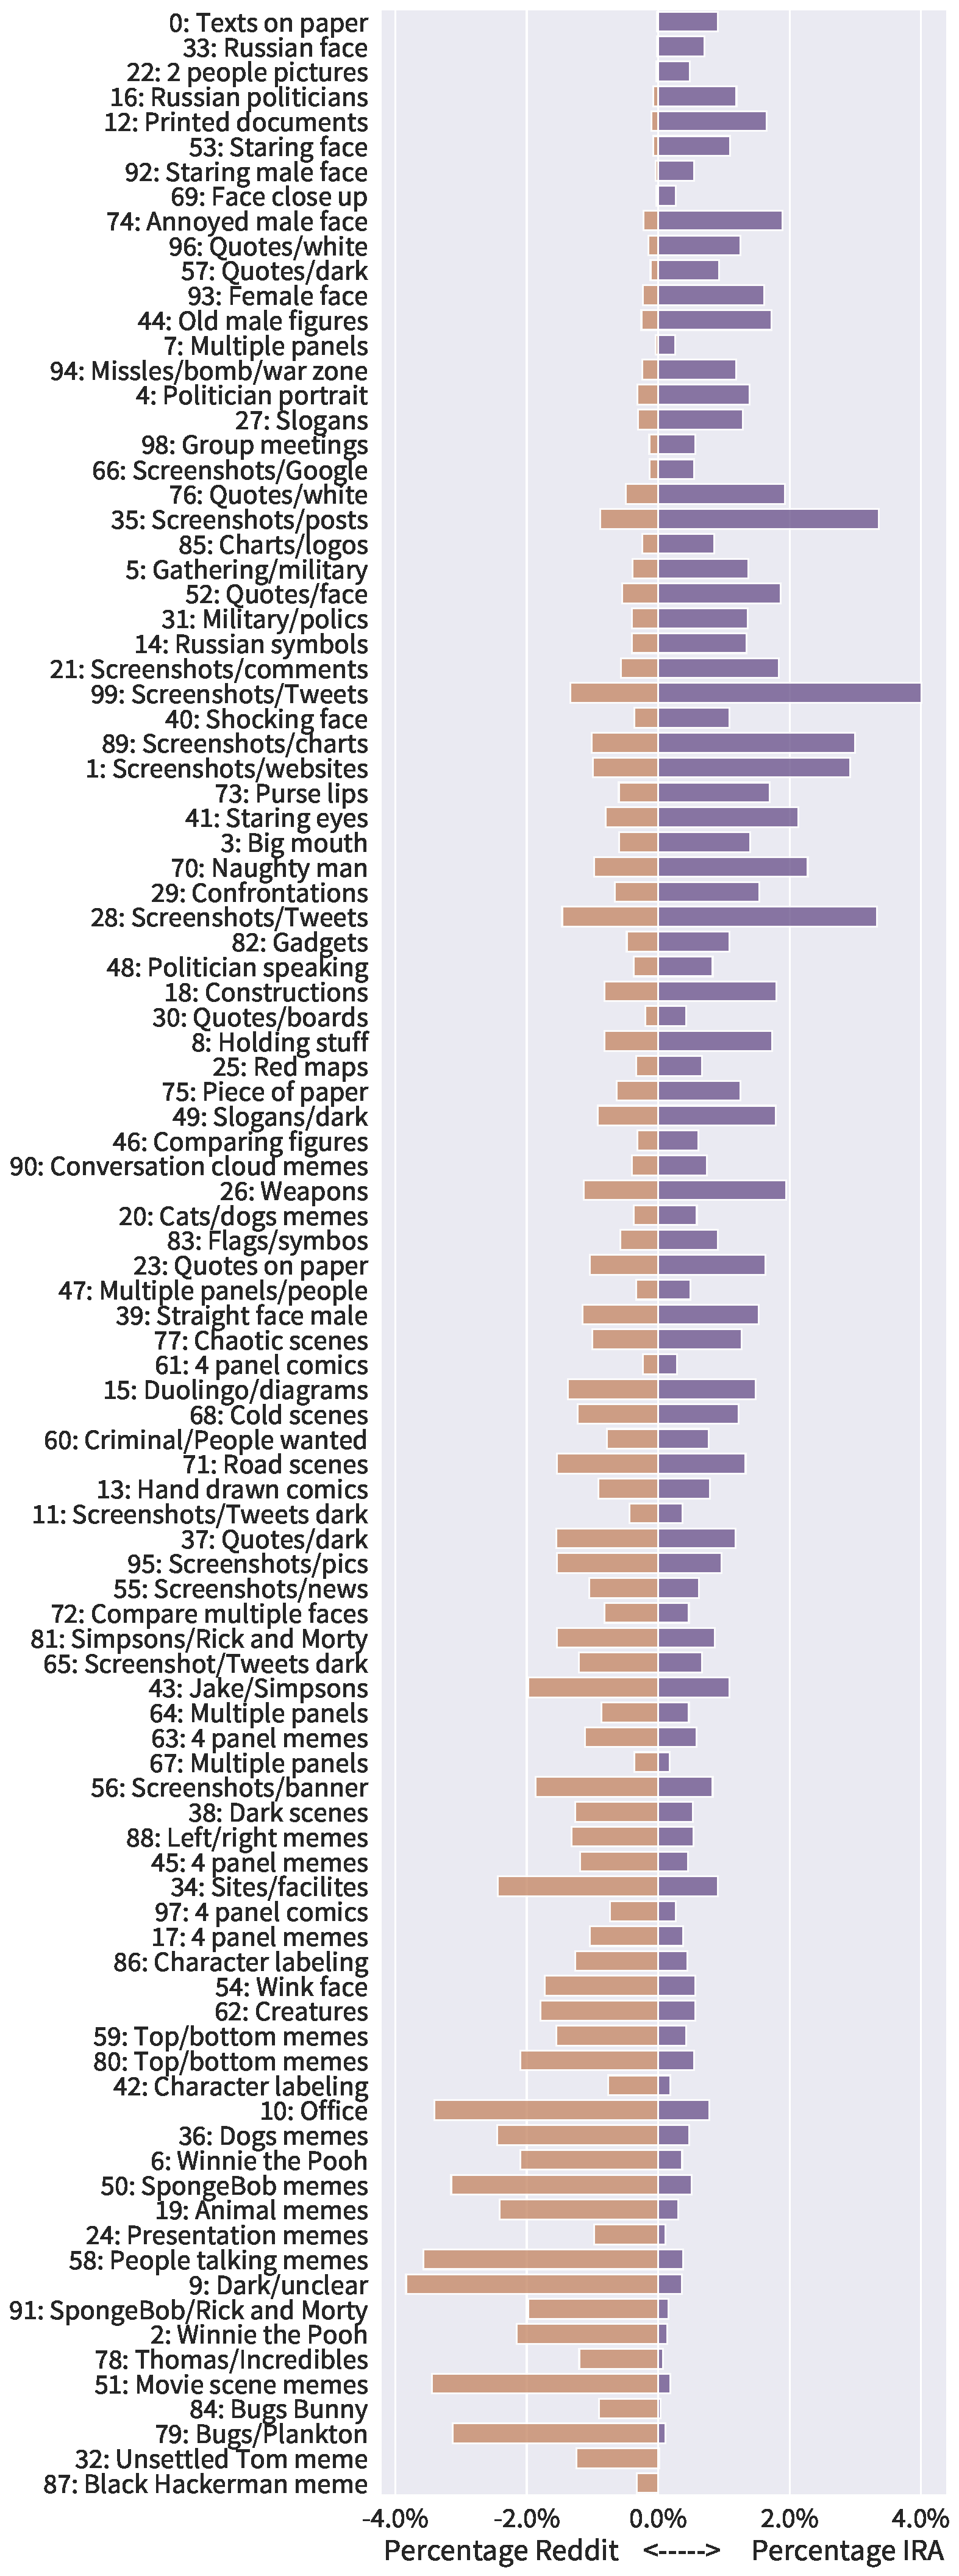
\includegraphics[width=.63\linewidth]{figure/cluster_share.pdf}
  \end{figure}
% \end{minipage}



\section{Next Steps}
\begin{adjustwidth}{0.1in}{0in}
\begin{enumerate}[topsep=0pt,itemsep=0ex,partopsep=0ex,parsep=0ex]
\item Compare with authentic memes on US Twitter or Russian social media
\item Use multimodal transformer (ex. VisualBERT) to extract embeddings that incorprate textual information and text-scene interactions
\item More flexible clustering models to incorporate tweet-level covariates
\end{enumerate} 
\end{adjustwidth}



%\hrule
\printbibliography[heading=none]


\end{adjmulticols*}
%------------------ Body End ---------------------%
%end the poster

\end{document}

